\documentclass[11pt,a4paper]{article}

\usepackage[margin=0.85in]{geometry}
\usepackage{graphicx}
\usepackage{booktabs}
\usepackage{amsmath}
\usepackage{listings}
\usepackage{xcolor}
\usepackage{float}
\usepackage{hyperref}
\usepackage{caption}
\usepackage{array}

\hypersetup{
    colorlinks=true,
    linkcolor=blue!60!black,
    urlcolor=blue!60!black,
    pdftitle={Systems Lab Report - Assignments and Group Project},
    pdfauthor={Ritam Ghosh, Aayush Dey, Abhirup Sarkar, Subhrojyoti Bala, Joydeep Baidya}
}

\definecolor{codebg}{rgb}{0.97,0.97,0.98}
\definecolor{codeframe}{rgb}{0.82,0.84,0.88}
\definecolor{codekw}{rgb}{0.10,0.28,0.62}
\definecolor{codecmt}{rgb}{0.36,0.44,0.36}
\definecolor{codestr}{rgb}{0.58,0.18,0.18}

\lstdefinestyle{x86asm}{
    backgroundcolor=\color{codebg},
    frame=single,
    rulecolor=\color{codeframe},
    basicstyle=\ttfamily\scriptsize,
    keywordstyle=\color{codekw}\bfseries,
    commentstyle=\color{codecmt}\itshape,
    stringstyle=\color{codestr},
    comment=[l];,
    morestring=[b]',
    morestring=[b]",
    breaklines=true,
    showstringspaces=false,
    tabsize=4,
    morekeywords={proc,endp,equ,db,dw,dup,near,far,mov,xor,add,sub,mul,div,shl,shr,cmp,jmp,je,jne,jb,jae,ja,jbe,jle,jge,jc,jnc,jnz,jz,jns,jcxz,call,ret,push,pop,pushf,popf,int,rep,repe,cmpsb,stosw,inc,dec,neg,and,or,test,loop,lea,cld,cli,hlt,offset,byte,word,ptr,end}
}

\lstset{style=x86asm}

\setlength{\parskip}{0.45em}
\setlength{\parindent}{0pt}

\begin{document}

% ============================================================================
% TITLE PAGE
% ============================================================================
\begin{titlepage}
    \centering
    \vspace*{0.8cm}
    {\large\scshape Systems Programming Laboratory --- Group Submission \par}
    \vspace{0.6cm}
    \rule{\linewidth}{0.6pt}\\[0.45cm]
    {\LARGE\bfseries Systems Programming Lab Report:\\[0.15cm]
    Part I: MASM Lab Assignments (10 Problems)\\[0.15cm]
    Part II: Real-Mode Maze System \& Extensions \par}
    \rule{\linewidth}{0.6pt}
    \vspace{0.9cm}

    {\normalsize\textbf{Part I --- Assignment Report:} Level~1 (5 Problems) and Level~2 (5 Problems) in 16-Bit 8086 MASM}\\[0.2cm]
    {\normalsize\textbf{Part II --- Group Project Report:} \texttt{Code/MAZE.ASM}, DOSBox-RS Emulator,\\
    Network PvP, Android Port, Cognitive Study CSV Telemetry, and Live Leaderboard}

    \vspace{1.2cm}

    {\large\bfseries Group Members \& Assignment Question Mapping}\\[0.4cm]
    \small
    \begin{tabular}{@{}llp{8.4cm}@{}}
        \toprule
        \textbf{Roll Number} & \textbf{Name} & \textbf{Assigned Questions (2 Consecutive Problems Each)} \\
        \midrule
        \texttt{002410501040} & Ritam Ghosh      & \textbf{Problems 1 \& 2} (Assignment~1: Q1, Q2) --- Block transfer ($5x+10$) from \texttt{3000H} to \texttt{4000H}; 20-element zig-zag array at \texttt{4000H}. \\[0.15cm]
        \texttt{002410501043} & Aayush Dey       & \textbf{Problems 3 \& 4} (Assignment~1: Q3, Q4) --- Hexadecimal-to-ASCII conversion; basic arithmetic calculator (\texttt{+}, \texttt{-}, \texttt{*}, \texttt{/}). \\[0.15cm]
        \texttt{002410501045} & Abhirup Sarkar   & \textbf{Problems 5 \& 6} (Assignment~1: Q5; Assignment~2: Q1) --- String operations library (\texttt{STRLEN}, \texttt{STRCMP}, \texttt{STRREV}); boot-level BIOS password verifier. \\[0.15cm]
        \texttt{002410501054} & Subhrojyoti Bala & \textbf{Problems 7 \& 8} (Assignment~2: Q2, Q3) --- DOS command-line shell emulator (\texttt{DIR}, \texttt{TYPE}, \texttt{COPY}, \texttt{EXIT}); FCFS disk scheduling calculator. \\[0.15cm]
        \texttt{002410501062} & Joydeep Baidya   & \textbf{Problems 9 \& 10} (Assignment~2: Q4, Q5) --- $n$-element signed array sorter; stack-based multi-bracket balancing verifier. \\
        \bottomrule
    \end{tabular}

    \vfill
    {\normalsize November 2026 \par}
\end{titlepage}

\tableofcontents
\newpage

% ============================================================================
% PART I: LAB ASSIGNMENTS REPORT
% ============================================================================
\part{Lab Assignments Report}

All ten problems across Assignment~1 (Level~1) and Assignment~2 (Level~2) target the 8086 real-mode \texttt{.MODEL SMALL} / \texttt{.STACK 100H} environment and were divided consecutively among the five group members (two problems per member).

% ----------------------------------------------------------------------------
% SECTION 1: ASSIGNMENT 1 (LEVEL 1)
% ----------------------------------------------------------------------------
\section{Assignment 1 (Level 1)}

% --- Problem 1 ---
\subsection{Problem 1 (Assignment 1, Q1) --- Ritam Ghosh (\texttt{002410501040})}

\textbf{Question:} Write an MASM program to transfer a block of 10 data bytes from one memory location, \texttt{3000H}, to another memory location, \texttt{4000H}. Before transfer, multiply 5, then add 10 to each element.

\textbf{Approach:} The program reads 10 single-digit numbers via \texttt{INT 21H / AH=01H}, converts ASCII characters to numeric bytes (\texttt{SUB AL, 30H}), and stores them starting at \texttt{DS:3000H}. A second loop indexed by \texttt{SI=3000H} and \texttt{DI=4000H} (\texttt{CX=0AH}) loads each byte into \texttt{AL}, computes \texttt{AL * 5} with \texttt{MUL BL} (\texttt{BL=05H}), adds \texttt{0AH}, writes the result to \texttt{[DI]}, and prints the transformed array using \texttt{PRINT\_NUM}.

\lstinputlisting[caption={Assignment 1, Q1 (\texttt{a1\_q1.asm}) --- Block transfer with $5x+10$ transformation.}]{assignments/a1_q1.asm}

% --- Problem 2 ---
\subsection{Problem 2 (Assignment 1, Q2) --- Ritam Ghosh (\texttt{002410501040})}

\textbf{Question:} Write an MASM program to store an array of 20 numbers in zig-zag (alternating less than and greater than) order in memory location \texttt{4000H}.

\textbf{Approach:} After reading 20 elements into \texttt{ARR} and copying them to \texttt{4000H}, a single $O(n)$ pass checks 19 adjacent pairs (\texttt{[SI]} and \texttt{[SI+1]}). Using \texttt{TEST BX, 01H} to distinguish even and odd indices, even positions enforce $a[i] \le a[i+1]$ and odd positions enforce $a[i] \ge a[i+1]$, swapping bytes whenever the inequality fails.

\lstinputlisting[caption={Assignment 1, Q2 (\texttt{a1\_q2.asm}) --- Single-pass $O(n)$ zig-zag array ordering at \texttt{4000H}.}]{assignments/a1_q2.asm}

% --- Problem 3 ---
\subsection{Problem 3 (Assignment 1, Q3) --- Aayush Dey (\texttt{002410501043})}

\textbf{Question:} Write an MASM program to convert a hexadecimal number into its equivalent ASCII.

\textbf{Approach:} Two hexadecimal characters are read via \texttt{AH=01H} and converted into 4-bit nibbles by \texttt{ASCII\_TO\_NIBBLE} (subtracting \texttt{30H} for \texttt{'0'--'9'}, or clearing bit~5 via \texttt{AND AL, 0DFH} and subtracting \texttt{37H} for \texttt{'A'--'F'}). Shifting the high nibble left by 4 (\texttt{SHL AL, CL}) and OR-ing the low nibble reconstructs the byte in \texttt{HEX\_NUM}, which is printed as its ASCII character via \texttt{AH=02H}.

\lstinputlisting[caption={Assignment 1, Q3 (\texttt{a1\_q3.asm}) --- Two-digit hexadecimal to ASCII converter.}]{assignments/a1_q3.asm}

% --- Problem 4 ---
\subsection{Problem 4 (Assignment 1, Q4) --- Aayush Dey (\texttt{002410501043})}

\textbf{Question:} Write an MASM program to implement a basic calculator for arithmetic operations.

\textbf{Approach:} The program reads two single-digit operands and an operator (\texttt{+}, \texttt{-}, \texttt{*}, \texttt{/}) via \texttt{AH=01H}, branching to the corresponding handler. Division checks \texttt{BL == 0} to trap divide-by-zero errors. In \texttt{DISPLAY\_RESULT}, bit~15 is tested (\texttt{TEST BX, 8000H}) to print a minus sign and negate negative subtraction results before outputting decimal digits from the stack.

\lstinputlisting[caption={Assignment 1, Q4 (\texttt{a1\_q4.asm}) --- Basic arithmetic calculator (\texttt{+}, \texttt{-}, \texttt{*}, \texttt{/}).}]{assignments/a1_q4.asm}

% --- Problem 5 ---
\subsection{Problem 5 (Assignment 1, Q5) --- Abhirup Sarkar (\texttt{002410501045})}

\textbf{Question:} Implement a library of string operations using assembly: (a) \texttt{STRLEN}: return length of string; (b) \texttt{STRCMP}: compare two strings; (c) \texttt{STRREV}: reverse string in place.

\textbf{Approach:} Strings are read via DOS buffered input (\texttt{AH=0AH}) and terminated with \texttt{'\$'} by \texttt{READ\_STRING}. \texttt{STRLEN} scans \texttt{[SI]} until \texttt{'\$'}, returning length in \texttt{CX}. \texttt{STRCMP} compares \texttt{[SI]} and \texttt{[DI]} byte-by-byte returning \texttt{AX=0} if equal or \texttt{1} otherwise. \texttt{STRREV} locates the last character before \texttt{'\$'} with \texttt{DI} and swaps \texttt{[SI]} and \texttt{[DI]} inward until the pointers meet.

\lstinputlisting[caption={Assignment 1, Q5 (\texttt{a1\_q5.asm}) --- String library implementing \texttt{STRLEN}, \texttt{STRCMP}, and \texttt{STRREV}.}]{assignments/a1_q5.asm}

% ----------------------------------------------------------------------------
% SECTION 2: ASSIGNMENT 2 (LEVEL 2)
% ----------------------------------------------------------------------------
\section{Assignment 2 (Level 2)}

% --- Problem 6 ---
\subsection{Problem 6 (Assignment 2, Q1) --- Abhirup Sarkar (\texttt{002410501045})}

\textbf{Question:} Boot-level password verification system: simulate a BIOS-like password verification system with: (a) accepting hidden password input (no echo), (b) comparing with a hardcoded value, (c) allowing up to 3 retries before locking, and (d) using BIOS interrupts for keyboard handling.

\textbf{Approach:} Rather than DOS echoed input, \texttt{input\_loop} reads keys silently with \texttt{INT 16h / AH=00h}, supporting Backspace (\texttt{08h}) and Enter (\texttt{0Dh}). Upon submission, length is checked against \texttt{pass\_len} and characters are compared against \texttt{hardcoded\_pass} using \texttt{CLD} + \texttt{REPE CMPSB} (\texttt{DS:SI} vs \texttt{ES:DI}). Three failed attempts clear \texttt{attempts} and enter a \texttt{CLI} / \texttt{HLT} system lock loop.

\lstinputlisting[caption={Assignment 2, Q1 (\texttt{a2\_q1.asm}) --- BIOS-level silent password verification with 3-retry lock.}]{assignments/a2_q1.asm}

% --- Problem 7 ---
\subsection{Problem 7 (Assignment 2, Q2) --- Subhrojyoti Bala (\texttt{002410501054})}

\textbf{Question:} Design and implement a simple command-line shell emulator using MASM that prompts for user commands and interprets \texttt{DIR} (mock file listing), \texttt{TYPE <filename>} (display file contents), \texttt{COPY <source> <destination>} (copy file contents), and \texttt{EXIT} (terminate), using DOS interrupts (\texttt{INT 21h}).

\textbf{Approach:} Lines read via \texttt{AH=0Ah} are null-terminated, stripped of leading spaces (\texttt{skip\_sp}), and matched against command keywords. \texttt{DIR} displays a preset listing; \texttt{EXIT} invokes \texttt{AH=4Ch}; \texttt{TYPE} opens \texttt{file1} (\texttt{AH=3Dh, AL=0}), reads 1 byte at a time (\texttt{AH=3Fh}) until \texttt{AX=0}, prints via \texttt{AH=02h}, and closes (\texttt{AH=3Eh}); \texttt{COPY} opens source (\texttt{3Dh}), creates destination (\texttt{3Ch}), and loops 128-byte \texttt{3Fh}/\texttt{40h} transfers before closing both handles.

\lstinputlisting[caption={Assignment 2, Q2 (\texttt{a2\_q2.asm}) --- Command-line DOS shell emulator (\texttt{DIR}, \texttt{TYPE}, \texttt{COPY}, \texttt{EXIT}).}]{assignments/a2_q2.asm}

% --- Problem 8 ---
\subsection{Problem 8 (Assignment 2, Q3) --- Subhrojyoti Bala (\texttt{002410501054})}

\textbf{Question:} Implement FCFS (First-Come-First-Served) disk scheduling algorithm using MASM.

\textbf{Approach:} Multi-digit integers are parsed by \texttt{read\_num} for \texttt{initial\_head}, request count \texttt{n}, and each word in \texttt{requests[]}. Iterating in arrival order, the loop computes seek distance $|r_i - \text{prev}|$ via \texttt{SUB AX, BX} followed by \texttt{JNS}/\texttt{NEG}, prints per-step movement and seek distance, accumulates \texttt{total\_mov}, and computes average head movement via \texttt{DIV BX} (guarded against $n=0$).

\lstinputlisting[caption={Assignment 2, Q3 (\texttt{a2\_q3.asm}) --- FCFS disk scheduling seek calculator.}]{assignments/a2_q3.asm}

% --- Problem 9 ---
\subsection{Problem 9 (Assignment 2, Q4) --- Joydeep Baidya (\texttt{002410501062})}

\textbf{Question:} Implement a MASM program to sort an array of $n$ elements ($n$ should be taken as user input).

\textbf{Approach:} The program reads \texttt{n} and \texttt{n} signed 16-bit elements into \texttt{array[]} using \texttt{read\_num} (which recognizes a leading \texttt{'-'} sign and applies two's-complement \texttt{NEG}). An $O(n^2)$ bubble sort compares adjacent words with signed \texttt{CMP AX, [SI+2]} and \texttt{JLE no\_swap}, swapping out-of-order pairs in place before printing the sorted array via \texttt{print\_num}.

\lstinputlisting[caption={Assignment 2, Q4 (\texttt{a2\_q4.asm}) --- Signed $n$-element bubble sort in 16-bit MASM.}]{assignments/a2_q4.asm}

% --- Problem 10 ---
\subsection{Problem 10 (Assignment 2, Q5) --- Joydeep Baidya (\texttt{002410501062})}

\textbf{Question:} Develop a MASM program that accepts a string consisting of multiple types of brackets (\texttt{()}, \texttt{\{\}}, \texttt{[]}) and verifies using a stack-based approach whether they are balanced and properly nested, outputting \texttt{Balanced} or \texttt{Non-Balanced}.

\textbf{Approach:} Reading one character at a time via \texttt{AH=01h} until Enter (\texttt{0Dh}), opening brackets are pushed onto \texttt{stack\_arr} indexed by \texttt{top}. Closing brackets invoke \texttt{pop\_char} to verify non-empty stack status (\texttt{AH=1}) and exact bracket-pair matching; non-bracket characters are skipped. At end of input, \texttt{top == 0} prints \texttt{Balanced}, while any mismatch, underflow, or leftover opening bracket prints \texttt{Non-Balanced}.

\lstinputlisting[caption={Assignment 2, Q5 (\texttt{a2\_q5.asm}) --- Stack-based bracket nesting verifier.}]{assignments/a2_q5.asm}

\newpage

% ============================================================================
% PART II: GROUP PROJECT REPORT
% ============================================================================
\part{Group Project Report: Real-Mode MASM Maze System}

\section{Problem Statement and Brief Theory}

\subsection{Base Project Objective}
The Systems Lab group project builds on the maze assignment specification: write a 16-bit MASM program to draw a navigable maze, place the player at a starting position, process arrow and \texttt{W/A/S/D} keyboard input through BIOS interrupts, enforce wall collisions so movement stays on open corridors, and update the display smoothly.

Starting from this base in \texttt{Code/MAZE.ASM}, we implemented a three-level random maze system ($15\times 15$, $24\times 24$, and $36\times 36$) supporting three modes: single-player race against a fair A* bot, two-player networked PvP, and a multi-stage cognitive study mode with automated CSV logging.

\subsection{Real-Mode Segmented Memory and BIOS/DOS Interrupts}
\texttt{MAZE.ASM} targets the 8086 real-mode \texttt{.model small} memory layout with a 512-byte stack (\texttt{.stack 200h}). Code resides in \texttt{CS}, static and working arrays reside in \texttt{DGROUP} addressed via \texttt{DS}, and \texttt{ES} is permanently pointed to segment \texttt{0B800h} (CGA/VGA color text video memory) inside \texttt{main}. Direct memory writes to \texttt{ES} avoid slower per-character BIOS teletype calls during active gameplay.

All hardware interaction goes through real-mode software interrupts, summarized in Table~\ref{tab:interrupts}.

\begin{table}[H]
    \centering
    \caption{Software interrupts used by \texttt{Code/MAZE.ASM}.}
    \label{tab:interrupts}
    \small
    \begin{tabular}{@{}lllp{6.4cm}@{}}
        \toprule
        \textbf{Vector} & \textbf{Function} & \textbf{Key Registers} & \textbf{Purpose in \texttt{MAZE.ASM}} \\
        \midrule
        \texttt{INT 10h} & \texttt{AH=00h} & \texttt{AL=03h} & Set $80\times 25$ 16-color text mode and clear screen. \\
        \texttt{INT 10h} & \texttt{AX=1003h} & \texttt{BL=00h} & Disable attribute blinking so bit~7 selects bright background colors (16 total). \\
        \texttt{INT 16h} & \texttt{AH=00h/01h} & \texttt{AH}=scan, \texttt{AL}=ASCII & Non-blocking poll (\texttt{01h}) in race loop; blocking read (\texttt{00h}) in menus and study mode. \\
        \texttt{INT 1Ah} & \texttt{AH=00h} & \texttt{CX:DX}=ticks & Read 18.2\,Hz BIOS timer ticks for PRNG seeding, countdowns, bot speed, and clocks. \\
        \texttt{INT 21h} & \texttt{AH=3Ch--42h} & \texttt{DS:DX}=path, \texttt{BX}=handle & Create, open, read, write, seek, and delete \texttt{MAZE.CFG}, \texttt{COGLOAD.TMP}, and \texttt{COGLOAD.CSV}. \\
        \texttt{INT 61h} & \texttt{AH=00h--05h} & \texttt{DS:SI/DI}, \texttt{CX}, \texttt{DX} & Custom DOSBox-RS WebSocket relay interface for networked PvP (mode~2). \\
        \bottomrule
    \end{tabular}
\end{table}

\subsection{Half-Block \texorpdfstring{$80\times 50$}{80x50} Square Pixel Rendering}
Standard DOS text mode (\texttt{03h}) provides only 25 rows, which cannot fit a $36\times 36$ maze at one row per cell. \texttt{MAZE.ASM} doubles vertical resolution by filling every maze cell with the CP437 upper-half block character (\texttt{0DFh}). In VGA text memory, each character cell occupies two bytes at \texttt{B800h}: the ASCII byte at even offset and the attribute byte at odd offset (low nibble = foreground, high nibble = background). With blinking disabled via \texttt{INT 10h AX=1003h BL=0}, setting \texttt{even y} in the low nibble and \texttt{odd y} in the high nibble yields an $80\times 50$ square-pixel framebuffer using only text mode.

% ============================================================================
% CORE IMPLEMENTATION (MAZE.ASM)
% ============================================================================
\section{Core Implementation (\texttt{Code/MAZE.ASM})}

\subsection{Flat Grid Representation and Memory Reuse}
To avoid repeated 2D multiply-and-add indexing in 8086 registers, the grid is stored as a flat row-major byte array \texttt{grid[MAXC]} where \texttt{MAXC = 36 * 36 = 1296}. Cell $(r, c)$ sits at linear index $i = r \cdot \texttt{msize} + c$. Directional offsets are kept in a 4-word table \texttt{deltas}:
\[
\texttt{deltas} = [-\texttt{msize}\ (\text{Up}),\ +\texttt{msize}\ (\text{Down}),\ -1\ (\text{Left}),\ +1\ (\text{Right})].
\]
Checking a neighbor becomes a single indexed addition (\texttt{add ax, deltas[bx]}). Furthermore, because maze construction finishes before the race begins, A* pathfinding reuses the build-time arrays through \texttt{EQU} aliases (\texttt{gcost equ dstart}, \texttt{closed equ mark}, \texttt{bucket0 equ queue}, \texttt{bucket1 equ dstack}), keeping total \texttt{DGROUP} usage well inside the 64\,KB real-mode segment limit.

\subsection{Maze Generation (\texttt{buildmaze}, \texttt{genmaze}, \texttt{carvable})}
Mazes are generated fresh on every level using a 16-bit linear congruential generator (\texttt{seed = seed * 25173 + 13849}), initialized from \texttt{INT 1Ah} (or synchronized from the server seed in PvP mode). Generation proceeds in four steps inside \texttt{buildmaze}:

\begin{enumerate}
    \item \textbf{Randomised DFS (\texttt{genmaze}):} All \texttt{cells} start as walls (\texttt{0}). Start square $(1,1)$ (\texttt{spos}) is carved (\texttt{1}) and pushed onto \texttt{dstack}. At each step, the top square tests all four \texttt{deltas}. A neighbor is valid (\texttt{carvable}) only if it lies strictly inside the outer wall border, is currently a wall, has exactly one open orthogonal neighbor (the cell we came from), and both squares diagonally ahead in the moving direction are walls. This invariant keeps all corridors strictly one square wide and yields a spanning tree (perfect maze). One valid neighbor is chosen at random; dead ends pop \texttt{dstack}.
    \item \textbf{Exit Placement (\texttt{placeexit}):} Scans all open squares and picks the square maximizing $\text{row} + \text{col}$, placing \texttt{epos} near the bottom-right corner.
    \item \textbf{Guaranteed Alternative Route (\texttt{countwalls} with \texttt{strict=1}):} Breadth-first search runs from \texttt{spos} into \texttt{dstart[]} and from \texttt{epos} into \texttt{dexit[]}. A square lies on a shortest route when $\texttt{dstart}[i] + \texttt{dexit}[i] = \texttt{pathlen}$. \texttt{checkwall} searches for an inner wall separating two opposite open cells that both lie on the shortest route and differ in \texttt{dexit} by at least 4 steps. Opening one such wall via \texttt{openrandom} guarantees at least two distinct paths to the exit (re-generating up to 50 times if none exists).
    \item \textbf{Extra Loops:} With \texttt{strict=0}, $\lfloor \texttt{msize}/2 \rfloor$ additional inner walls between opposite open cells are opened to create tactical loops, followed by a final \texttt{bfs} from \texttt{epos} to finalize \texttt{dexit[]}.
\end{enumerate}

\subsection{Optimal Path Calculation and Fair A* Opponent}
The exact optimal distance table \texttt{dexit[]} is computed once per maze via \texttt{bfs} in $O(V)$ time using the circular queue \texttt{queue[]}. Every open square stores its exact shortest step count to the exit (\texttt{0FFFFh} if unreachable). This table drives four subsystems:
\begin{itemize}
    \item \textbf{Live Distance HUD:} Displays remaining optimal steps (\texttt{Dist}) under each player's maze.
    \item \textbf{Time-Out Arbitration:} When the level timer (\texttt{30/45/60\,s} = \texttt{546/819/1092} BIOS ticks) expires, whoever has smaller \texttt{dexit[ppos]} wins.
    \item \textbf{Hint Overlay (\texttt{showhint}):} Pressing \texttt{H} or \texttt{ENTER} walks greedily from the player's square to any open neighbor with \texttt{dexit[nbr] == cur - 1}, painting the shortest path in cyan (\texttt{C\_HINT}) until the next move.
    \item \textbf{Post-Level Optimal Trace (\texttt{tracepath}):} Marks one shortest path in \texttt{mark[]} so \texttt{showresult} renders optimal squares in yellow, walked squares in red, and overlap in orange.
\end{itemize}

\textbf{Two-Bucket A* Computer Bot (\texttt{botlook}, \texttt{botplan}):} To keep single-player races fair, the bot never inspects \texttt{dexit[]} or unseen parts of \texttt{grid[]}. It maintains its own map \texttt{known[]} initialized with unknown (\texttt{0}) inside and walls (\texttt{2}) along the border. After each move, \texttt{botlook} uncovers squares within Chebyshev radius \texttt{botsee} ($2, 3, 4$ by level) and sets \texttt{newwall = 1} if an unrecorded wall appears. Whenever \texttt{newwall = 1}, \texttt{botplan} replans using A* with Manhattan heuristic $h = |r - r_{\text{exit}}| + |c - c_{\text{exit}}|$ under the free-space assumption (unseen cells treated as open). Because each unit grid step increases $g$ by $1$ and changes $h$ by $\pm 1$, $f = g + h$ only changes by $0$ or $+2$ from the current minimum $f$. Consequently, \texttt{botplan} avoids a binary heap entirely and uses just two stack arrays---\texttt{bucket0} (current $f$) and \texttt{bucket1} ($f+2$)---running in linear time per replan.

\begin{figure}[H]
    \centering
    \begin{minipage}[t]{0.48\textwidth}
        \centering
        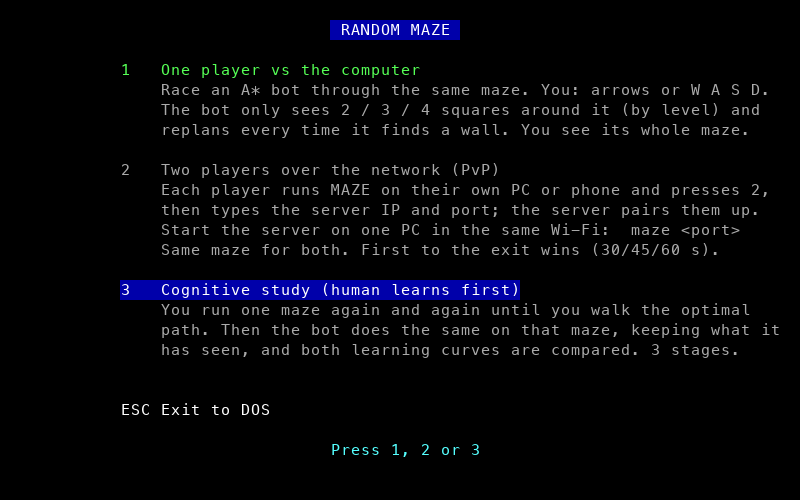
\includegraphics[width=\linewidth]{figures/fig_menu.png}
        \caption{Main menu of \texttt{MAZE.EXE} running inside DOSBox-RS, offering modes 1, 2, and 3.}
        \label{fig:menu}
    \end{minipage}\hfill
    \begin{minipage}[t]{0.48\textwidth}
        \centering
        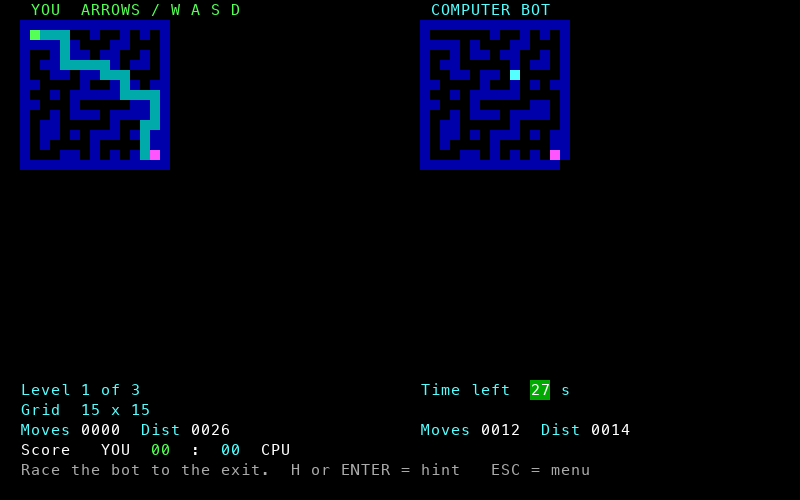
\includegraphics[width=\linewidth]{figures/fig_mode1_race.png}
        \caption{Mode~1 race ($15\times 15$): cyan hint path on left; A* bot advancing on right.}
        \label{fig:mode1}
    \end{minipage}
\end{figure}

\subsection{Important Code Segments}

\textbf{1. Direct Video RAM Half-Block Pixel Writer (\texttt{setpix}):}
\begin{lstlisting}[caption={Writing half-block square pixels straight into \texttt{B800h} text video memory.}]
setpix proc
    push ax
    push bx
    push cx
    mov cl,al                   ; CL = 4-bit VGA colour
    mov al,dh
    shr al,1                    ; text row = y / 2
    mov bl,160
    mul bl
    mov bx,ax
    mov al,dl
    xor ah,ah
    shl ax,1
    add bx,ax                   ; BX = byte offset in B800h
    mov byte ptr es:[bx],0DFh   ; CP437 upper half block
    mov al,es:[bx+1]
    test dh,1
    jnz sp_lower
    and al,0F0h                 ; even y -> low nibble (foreground)
    or al,cl
    jmp sp_store
sp_lower:
    and al,0Fh                  ; odd y  -> high nibble (background)
    shl cl,1
    shl cl,1
    shl cl,1
    shl cl,1
    or al,cl
sp_store:
    mov es:[bx+1],al
    pop cx
    pop bx
    pop ax
    ret
setpix endp
\end{lstlisting}

\textbf{2. Breadth-First Search Shortest-Distance Table (\texttt{bfs}):}
\begin{lstlisting}[caption={Linear-time BFS populating \texttt{dstart[]} or \texttt{dexit[]} from source \texttt{AX}.}]
bf_loop:
    mov si,qhead
    cmp si,qtail
    jae bf_done                 ; queue empty
    shl si,1
    mov ax,queue[si]
    inc qhead
    mov bx,ax
    shl bx,1
    mov dx,[di+bx]
    inc dx                      ; distance for adjacent squares
    xor cx,cx
bf_dir:
    mov bx,cx
    mov si,ax
    add si,deltas[bx]           ; neighbour index
    cmp grid[si],1
    jne bf_next
    mov bx,si
    shl bx,1
    cmp word ptr [di+bx],0FFFFh
    jne bf_next
    mov [di+bx],dx
    mov bx,qtail
    shl bx,1
    mov queue[bx],si
    inc qtail
bf_next:
    add cx,2
    cmp cx,8
    jb bf_dir
    jmp bf_loop
\end{lstlisting}

\textbf{3. Two-Bucket A* Expansion (\texttt{botplan}):}
\begin{lstlisting}[caption={Bucket swap and $f / f+2$ neighbor insertion in \texttt{botplan}.}]
bp_swap:
    mov ax,curp                 ; advance to f + 2 bucket
    xchg ax,nxtp
    mov curp,ax
    mov ax,nxtc
    mov curc,ax
    mov nxtc,0
    add curf,2
...
    call hcost
    add ax,dx                   ; AX = g + h = f(neighbour)
    cmp ax,curf
    mov ax,si
    je bp_same
    call pushnext               ; f = curf + 2
    jmp bp_pushed
bp_same:
    call pushcur                ; f = curf
\end{lstlisting}

\textbf{4. Cognitive Load LRUD Recording (\texttt{cogrec}):}
\begin{lstlisting}[caption={Capturing directional moves (\texttt{U/D/L/R}) in cognitive study mode.}]
cogrec proc                     ; record move from DX -> SI
    push ax
    push bx
    mov ax,si
    sub ax,dx
    cmp ax,deltas[0]
    jne cr_dn
    mov al,'U'
    jmp cr_put
cr_dn:
    cmp ax,deltas[2]
    jne cr_lf
    mov al,'D'
    jmp cr_put
cr_lf:
    cmp ax,deltas[4]
    jne cr_rt
    mov al,'L'
    jmp cr_put
cr_rt:
    cmp ax,deltas[6]
    jne cr_done
    mov al,'R'
cr_put:
    mov bx,movelen
    cmp bx,MAXMOV
    jae cr_done
    mov movebuf[bx],al
    inc movelen
cr_done:
    pop bx
    pop ax
    ret
cogrec endp
\end{lstlisting}

% ============================================================================
% ADDITIONAL WORKS
% ============================================================================
\section{Additional Works}

\subsection{Custom DOSBox-RS 8086 Emulator and Build Pipeline (\texttt{dosbox/})}
Rather than relying solely on external binary emulators that lack programmable networking, we built a self-contained 16-bit 8086 PC emulator in Rust (\texttt{dosbox/}) with zero third-party crate dependencies (\texttt{Cargo.toml} has an empty \texttt{[dependencies]} section).

\begin{itemize}
    \item \textbf{Emulated Hardware \& OS Layers:} \texttt{src/cpu/} implements the 8086 register file, flags, ModR/M decoding, ALU/BCD/mul-div, string operations, and 80186 extensions (\texttt{PUSHA/POPA}, \texttt{ENTER/LEAVE}, immediate shifts). \texttt{src/hardware/} models 1\,MB physical memory, $80\times 25$ video RAM at \texttt{B800:0000}, keyboard buffer, and PIT/clock state. \texttt{src/bios/} and \texttt{src/dos/} implement \texttt{INT 10h/15h/16h/1Ah} and \texttt{INT 21h} file I/O (\texttt{39h--47h}, \texttt{56h}), directory mapping onto a host folder mounted as \texttt{C:}, and MZ \texttt{.EXE} loading.
    \item \textbf{Built-In \texttt{MASM} and \texttt{LINK}:} \texttt{src/masm/} provides a multi-pass assembler supporting simplified/full segments, procedures, expressions, and automatic near-branch expansion when conditional jumps exceed $\pm 127$ bytes; \texttt{src/linker/} emits DOS \texttt{.EXE}, \texttt{.COM}, and \texttt{.MAP} files directly inside the DOS shell (\texttt{src/shell/}).
    \item \textbf{Terminal \& Headless Automation:} \texttt{src/terminal/} renders CP437 glyphs and 24-bit ANSI colors in terminal mode and also supports \texttt{--headless --keys --screenshot} for automated testing and HTML screen captures.
\end{itemize}

\textbf{Local Build and Execution:}
\begin{verbatim}
cargo build --release --manifest-path dosbox/Cargo.toml
dosbox/target/release/dosbox Code -c "masm MAZE.ASM;" -c "link MAZE.OBJ;" -c MAZE
\end{verbatim}

\subsection{Network PvP Architecture and Gameplay (Mode 2)}
Standard MS-DOS provides no TCP/IP socket stack. To enable real-time head-to-head racing across machines, DOSBox-RS exposes a custom software interrupt service on \texttt{INT 61h} via \texttt{service.rs} and \texttt{websocket.rs} inside \texttt{dosbox/src/net/}:

\begin{itemize}
    \item \textbf{Interrupt API:} \texttt{AH=00h} checks driver presence (returns \texttt{AX=4E57h}, \texttt{"NW"}); \texttt{AH=01h} initiates a non-blocking WebSocket handshake to \texttt{DS:SI} on port \texttt{DX}; \texttt{AH=02h} returns link state (\texttt{0}=closed, \texttt{1}=connecting, \texttt{2}=open, \texttt{3}=failed); \texttt{AH=03h} sends \texttt{CX} bytes from \texttt{DS:SI}; \texttt{AH=04h} pops a received frame into \texttt{DS:DI}; and \texttt{AH=05h} closes the socket. Server IP and port are saved in \texttt{C:\textbackslash MAZE.CFG} by \texttt{loadcfg}/\texttt{savecfg}.
    \item \textbf{Binary WebSocket Relay Protocol:} Defined identically in \texttt{server/src/protocol.rs} and \texttt{MAZE.ASM}: \texttt{Q} enters matchmaking; \texttt{M slot seedLo seedHi} pairs two players with the same 16-bit maze seed; \texttt{Y level} reports level readiness; \texttt{G level} starts the synchronized countdown; \texttt{O sqLo sqHi} relays each move coordinate in real time to the opponent's right-hand maze; \texttt{F level} reports exit arrival; \texttt{D level distLo distHi} sends remaining \texttt{dexit} distance on timeout; \texttt{R level winner reason} broadcasts the authoritative verdict; and \texttt{X} signals opponent disconnect.
\end{itemize}

\subsection{Android Mobile Build (\texttt{dosbox/android/})}
To run the same assembly program and network PvP on phones, the Rust emulator core was packaged as a native Android library under \texttt{dosbox/android/}:

\begin{itemize}
    \item \textbf{Zero-Dependency JNI Bridge (\texttt{native/src/}):} Built for \texttt{aarch64}, \texttt{armv7}, and \texttt{x86\_64} Android targets using NDK \texttt{27.1.12297006}. \texttt{jni.rs} implements direct JNI wrappers without third-party crates, \texttt{session.rs} runs the DOS thread (automatically assembling \texttt{MAZE.ASM} on first launch or whenever the bundled source updates), and \texttt{bridge.rs} shares the $80\times 25$ video buffer and key queue with the UI thread.
    \item \textbf{Handheld UI \& Controls (\texttt{app/.../dosbox/}):} \texttt{ScreenView.java} draws CP437 glyphs (\texttt{Cp437.java}) and 16-color palettes (\texttt{Palette.java}) onto an off-screen $1280\times 800$ bitmap refreshed at 60\,Hz with double-tap ($2.2\times$) and pinch-to-zoom ($4\times$). \texttt{ControllerView.java} and \texttt{DpadView.java} map touch controls to DOS scan codes (\texttt{D-pad} $\to$ arrows, \texttt{LEFT/RIGHT/START} $\to$ \texttt{1/2/3}, \texttt{A} $\to$ \texttt{ENTER}/hint, \texttt{B} $\to$ \texttt{ESC}, \texttt{SELECT} $\to$ soft keyboard, fast-forward $\to$ $1\times / 2\times / 4\times$ clock speed). \texttt{DriveFiles.java} manages import/export into the phone's \texttt{C:} storage. Built via \texttt{gradlew assembleRelease}.
\end{itemize}

\subsection{Cognitive Study Mode (Mode 3) and Stored Statistics (\texttt{COGLOAD.CSV})}
Mode~3 compares human spatial learning against the limited-sight A* bot across three stages ($15\times 15$, $24\times 24$, $36\times 36$) on identical mazes:
\begin{enumerate}
    \item \textbf{Human First (\texttt{runner=1}):} The participant walks from \texttt{spos} to \texttt{epos} repeatedly until completing one attempt in exactly \texttt{optlen} steps. Earlier attempts' trails are wiped on each new try (\texttt{cc\_study} hides \texttt{C\_OLD} when \texttt{runner != 0}), forcing recall from memory rather than visual tracing.
    \item \textbf{Bot Second (\texttt{runner=0}, \texttt{stview=1}):} The bot runs the same maze with sight radius~1, keeping its discovered \texttt{known[]} map across attempts. Once a try discovers no new walls, its initial optimistic plan equals the true shortest path, guaranteeing convergence.
\end{enumerate}

\begin{figure}[H]
    \centering
    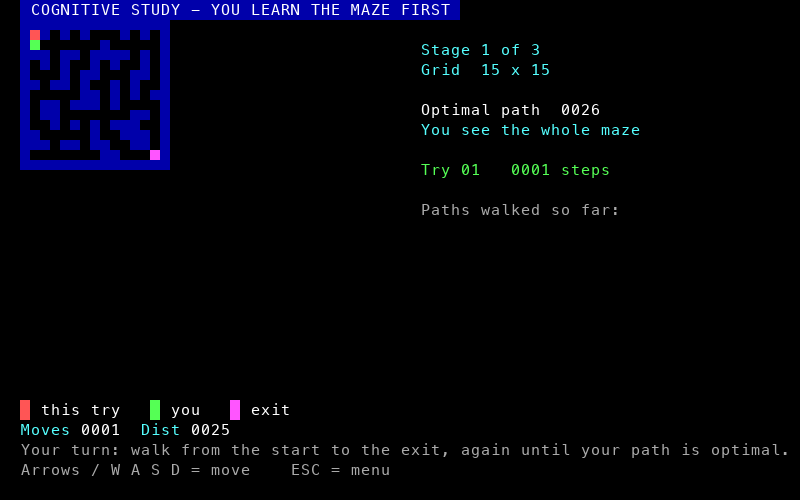
\includegraphics[width=0.76\linewidth]{figures/fig_mode3_study.png}
    \caption{Mode~3 Cognitive Study screen during human learning (Stage~1, $15\times 15$, optimal path 26 steps).}
    \label{fig:mode3}
\end{figure}

\textbf{Automated CSV Telemetry Pipeline:} Whenever \texttt{players == 3}, \texttt{applymove} invokes \texttt{cogrec}, storing each step as \texttt{L}, \texttt{R}, \texttt{U}, or \texttt{D} in \texttt{movebuf} (up to \texttt{MAXMOV = 4096} steps). At the end of each attempt (\texttt{endtry}), \texttt{cogtmp\_add} appends a compact 7-byte header plus the move string to \texttt{COGLOAD.TMP}. Once both human and bot finish the stage (\texttt{studycmp}), \texttt{cogsave} appends complete comparison rows to \texttt{C:\textbackslash COGLOAD.CSV} via \texttt{INT 21h} (\texttt{3Ch/3Dh/40h/42h}) and deletes \texttt{COGLOAD.TMP}.

Table~\ref{tab:cogload} summarizes the recorded comparison dataset stored in \texttt{Code/COGLOAD.CSV} across four mazes and all three grid stages.

\begin{table}[H]
    \centering
    \caption{Summary of cognitive load study records stored in \texttt{Code/COGLOAD.CSV}.}
    \label{tab:cogload}
    \scriptsize
    \resizebox{\textwidth}{!}{%
    \begin{tabular}{@{}cccccccll@{}}
        \toprule
        \textbf{Maze ID} & \textbf{Stage} & \textbf{Grid} & \textbf{Optimal} & \textbf{Runner} & \textbf{Attempt} & \textbf{Moves} & \textbf{Extra} & \textbf{Moves Sample (LRUD)} \\
        \midrule
        19482 & 1 & $15\times 15$ & 24 & player   & 1 / 2 & 30 & +6  & \texttt{RRDDDRRLRRDDDDDDRRRRRRRUUDDDDD} \\
        19482 & 1 & $15\times 15$ & 24 & player   & 2 / 2 & 24 & +0  & \texttt{RRDDDRRRDDDDDDRRRRRRRDDD} \\
        19482 & 1 & $15\times 15$ & 24 & computer & 1 / 3 & 36 & +12 & \texttt{RRDDDRRRUUDDDDDDRRRRRLLRRRRUUDDDDDDD} \\
        19482 & 1 & $15\times 15$ & 24 & computer & 3 / 3 & 24 & +0  & \texttt{RRDDDRRRDDDDDDRRRRRRRDDD} \\
        \midrule
        38353 & 1 & $15\times 15$ & 25 & player   & 1 / 3 & 37 & +12 & \texttt{RDDDLRRDRRURUDLDLLDDDDRDRRRDDRRRDRRUR} \\
        38353 & 1 & $15\times 15$ & 25 & player   & 3 / 3 & 25 & +0  & \texttt{RDDDRDDDDDRDRRRDDRRRDRRUR} \\
        38353 & 1 & $15\times 15$ & 25 & computer & 1 / 2 & 31 & +6  & \texttt{RRRRDRDDLDLLDDRRRRRDDRRDDDDRRUR} \\
        38353 & 1 & $15\times 15$ & 25 & computer & 2 / 2 & 25 & +0  & \texttt{RDDDRDDDRRRRRDDRRDDDDRRUR} \\
        \midrule
        53949 & 2 & $24\times 24$ & 61 & player   & 1 / 3 & 75 & +14 & \texttt{RDDLRRRDDLDLLUDRRDDLLUUUDDDDDRRRRURUUUR...} \\
        53949 & 2 & $24\times 24$ & 61 & player   & 3 / 3 & 61 & +0  & \texttt{RDDRRDDLDDDLLDDRRRRURUUURURRRDDRRRRRDDD...} \\
        53949 & 2 & $24\times 24$ & 61 & computer & 1 / 1 & 61 & +0  & \texttt{RDDRRDDLDDDLLDDRRRRURUUURURRRRRRRDDRDDD...} \\
        \midrule
        41892 & 3 & $36\times 36$ & 78 & player   & 1 / 3 & 94 & +16 & \texttt{RRRRDDLLRRDDDDDDRRRRRRUULLDDDRRUUURRRRR...} \\
        41892 & 3 & $36\times 36$ & 78 & player   & 3 / 3 & 78 & +0  & \texttt{RRRRDDDDDDDDDRRRRRRUUURRRRRDDDDDDRRRRRR...} \\
        41892 & 3 & $36\times 36$ & 78 & computer & 1 / 4 & 94 & +16 & \texttt{RRRRDDDDDDRRUULLDDDDDRRRRRRUUURRRRRDDDD...} \\
        41892 & 3 & $36\times 36$ & 78 & computer & 4 / 4 & 78 & +0  & \texttt{RRRRDDDDDDDDDRRRRRRUUURRRRRDDDDDDRRRRRR...} \\
        \bottomrule
    \end{tabular}%
    }
\end{table}

\subsection{PvP Server and Live Tournament Leaderboard (\texttt{server/})}
The PvP relay server (\texttt{server/src/}) is also written in dependency-free Rust, built via \texttt{cargo build --release --manifest-path server/Cargo.toml}. A single TCP listener handles both WebSocket PvP clients and standard HTTP browser requests:
\begin{itemize}
    \item \textbf{HTTP Dashboard \& JSON API:} Requests to \texttt{http://<server-ip>:<port>/} receive a live auto-refreshing (5\,s) HTML ranking table rendered by \texttt{Leaderboard::generate\_html()}; requests to \texttt{/leaderboard.json} or \texttt{/api} return structured JSON. State persists across restarts via \texttt{leaderboard.json} and \texttt{leaderboard.txt}, and an ASCII table prints to the server terminal after each level and match.
    \item \textbf{Scoring Metric:} To reward fast completion as well as closeness on timeouts, total score is computed as:
    \[
    \text{Score} = 150 W_{\text{match}} + 50 D_{\text{match}} + 100 W_{\text{exit}} + 60 W_{\text{time}} + 30 D_{\text{level}} + 10 N_{\text{levels}} + \text{SpeedBonus},
    \]
    where $\text{SpeedBonus}$ adds $+1$ point per second remaining on the level clock when reaching the exit. Ties break sequentially on total points, match wins, exit finishes, match win rate, and fewer losses.
\end{itemize}

\begin{figure}[H]
    \centering
    \begin{minipage}[t]{0.48\textwidth}
        \centering
        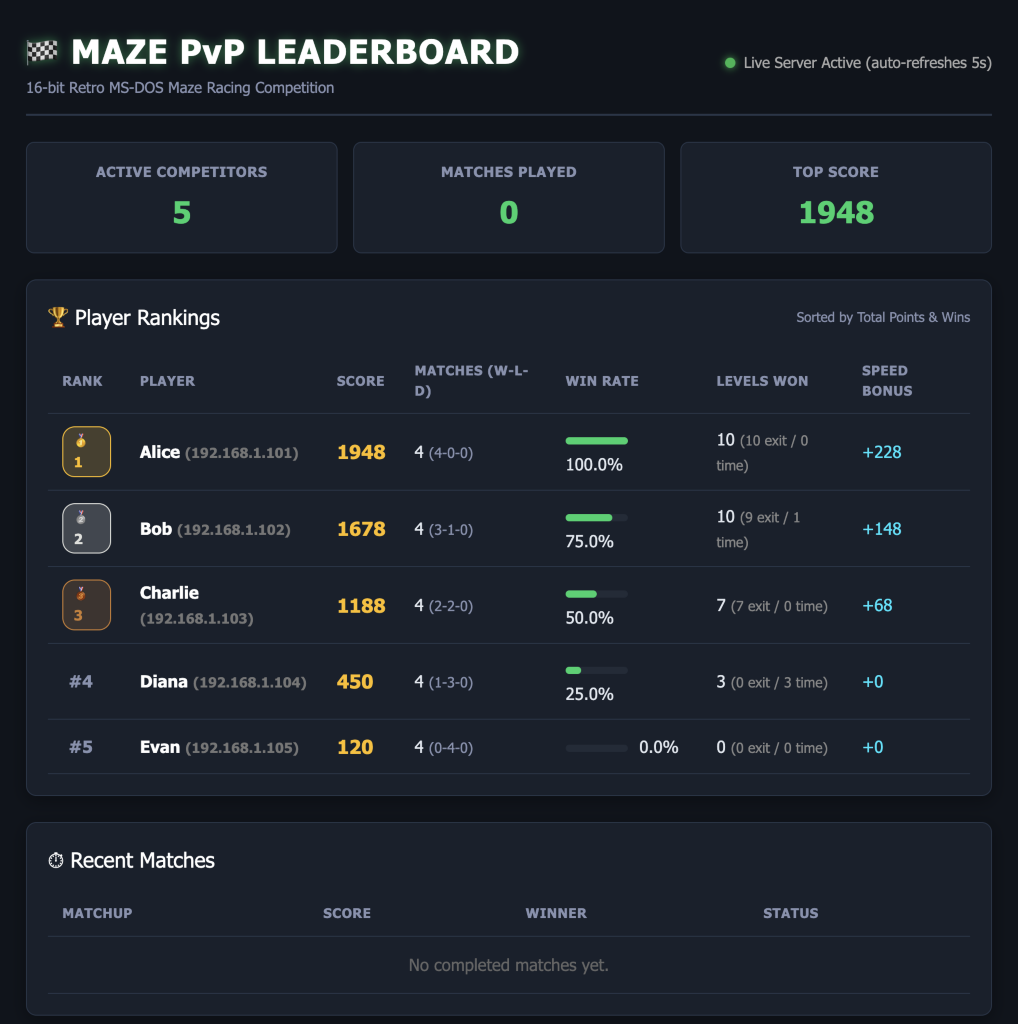
\includegraphics[width=\linewidth]{figures/fig_leaderboard_top.png}
        \caption{Live web leaderboard dashboard header, summary metrics, and player rankings.}
        \label{fig:lb_top}
    \end{minipage}\hfill
    \begin{minipage}[t]{0.48\textwidth}
        \centering
        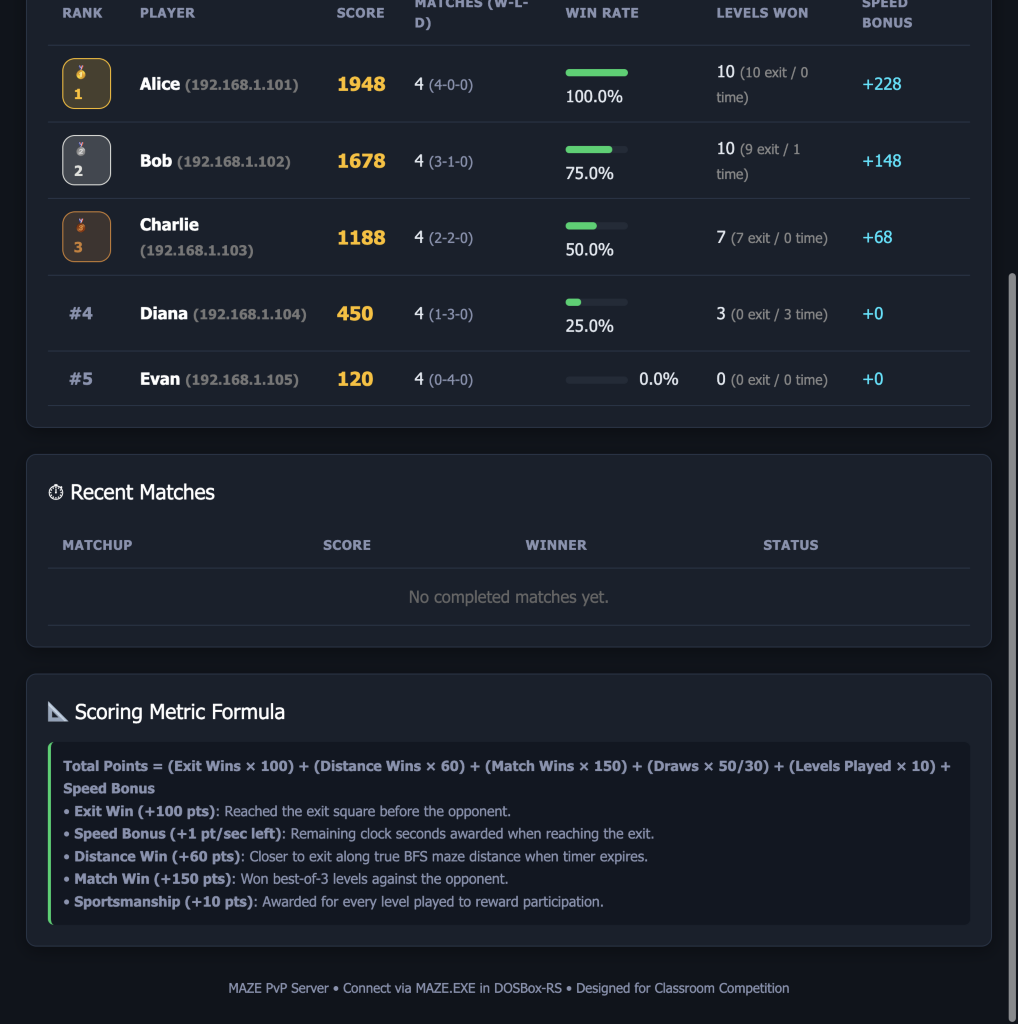
\includegraphics[width=\linewidth]{figures/fig_leaderboard_bottom.png}
        \caption{Dashboard lower section showing recent matches and scoring metric breakdown.}
        \label{fig:lb_bot}
    \end{minipage}
\end{figure}

% ============================================================================
% MEMBER CONTRIBUTIONS
% ============================================================================
\section{Member Contributions}

Table~\ref{tab:contributions} summarizes both the assignment problem split (Part~I) and the group project subsystem responsibilities (Part~II) across all five group members.

\begin{table}[H]
    \centering
    \caption{Group member assignments and project module contributions.}
    \label{tab:contributions}
    \small
    \begin{tabular}{@{}llp{9.0cm}@{}}
        \toprule
        \textbf{Roll Number} & \textbf{Name} & \textbf{Assignments \& Group Project Contributions} \\
        \midrule
        \texttt{002410501040} & Ritam Ghosh      & \textbf{Assignments:} A1 Q1, Q2. \textbf{Project:} Core 16-bit MASM game engine (\texttt{Code/MAZE.ASM}: maze generation, BFS, half-block renderer, A* opponent) and Android mobile build (\texttt{dosbox/android/}: JNI bridge, touch controller, handheld display). \\[0.1cm]
        \texttt{002410501043} & Aayush Dey       & \textbf{Assignments:} A1 Q3, Q4. \textbf{Project:} Cognitive study gameplay (Mode~3) and comparison metrics (learning-curve comparison tables and CSV telemetry evaluation). \\[0.1cm]
        \texttt{002410501045} & Abhirup Sarkar   & \textbf{Assignments:} A1 Q5; A2 Q1. \textbf{Project:} Custom 8086 DOSBox-RS emulator (\texttt{dosbox/}: CPU/BIOS/DOS core, built-in MASM/LINK) and networked PvP subsystem (\texttt{INT 61h} service, Mode~2 relay). \\[0.1cm]
        \texttt{002410501054} & Subhrojyoti Bala & \textbf{Assignments:} A2 Q2, Q3. \textbf{Project:} Core 16-bit MASM game engine (\texttt{Code/MAZE.ASM}) and live tournament leaderboard server (\texttt{server/}: scoring metric, ASCII console table, JSON/HTML dashboard). \\[0.1cm]
        \texttt{002410501062} & Joydeep Baidya   & \textbf{Assignments:} A2 Q4, Q5. \textbf{Project:} Cognitive study gameplay (Mode~3) and comparison metrics (attempt tracking, LRUD logging, and stage comparison analysis). \\
        \bottomrule
    \end{tabular}
\end{table}

\end{document}
